\documentclass[titlepage]{jsarticle}
\usepackage[dvipdfmx]{graphicx}
\usepackage{ascmac}
\usepackage{url}
\usepackage{listing}
\title{実施状況報告書}

\author{グループ番号:20 \\ 構成員:原口 卓也(1029285143) \\ 宮城 竜大(1029287621)}
\date{提出期限:2018年 5月10日 \\ 提出:\today}
\begin{document}
\maketitle
\section{現在の進捗状況}
\subsection{プロセッサの外部仕様}

SIMPLEアーキテクチャの仕様に沿ってプロセッサを実装した。
ほぼすべての機能がSIMPLEアーキテクチャと同じだが、シフト演算に限り、SIMPLEの設計仕様書の内容と異なる設計を行った。
これに関しては1.1.3で説明する。

\subsubsection{入力信号}

\begin{itemize}
\item clock:動作クロック。周波数はクロック用ロータリースイッチで定める。
\item reset:リセット信号。テンキースイッチA1を押すと、プロセッサの各レジスタの値がリセットされる。
\item exec:起動・停止信号。テンキースイッチA0を押して、プロセッサを起動・停止させる。
\item wren:デバッグ用の書き込み許可信号。命令メモリに書き込みを行うことはないので、最終報告ではGNDに置き換える予定。
\item in[15:0]:入力命令の入力値。ディップスイッチを16個用いて、16ビットの入力値を定める。A0が最上位ビットで、B7が最下位ビット。
\end{itemize}

\subsubsection{出力信号}

\begin{itemize}
\item clock\_out:動作クロックの出力。LED 0がクロックに合わせて点滅する。
\item phase1\verb|~|5:phase値の出力。phase1が実行中ならLED 1が点滅し、phase2ならLED 2が点滅、以下同様にして、実行中のphaseをLEDの点滅で知らせる。
\item PC\_check[31:0]:プログラム・カウンタの値を7セグメントLED A4\verb|~|A7に16進数表記で表示する。
\item LED[31:0]:出力命令の出力値を7セグメントLED A0\verb|~|A3に16進数表記で表示する。
\item selecter:点灯する7セグメントLEDの列を決定する。現状では、A列のみが光るようになっている。
\end{itemize}

\subsubsection{命令の種類}

\begin{enumerate}
\item 演算・入出力命令
\begin{itemize}
\item ADD Rd,RS:算術加算(r[Rd] = r[Rd] + r[Rs])
\item SUB Rd,Rs:算術減算(r[Rd] = r[Rd] - r[Rs])
\item AND Rd,RS:論理積 (r[Rd] = r[Rd] \& r[Rs])
\item OR Rd,Rs:論理和(r[Rd] = r[Rd] \verb+|+ r[Rs])

\item XOR Rd,RS:排他的論理和(r[Rd] = r[Rd] \verb|^| r[Rs])
\item CMP Rd,Rs:比較演算(r[Rd] - r[Rs]):条件コードの設定のみ行う
\item MOV Rd,RS:移動演算(r[Rd] = r[Rs])
\item SLL Rd,Rs,d:左論理シフト(r[Rd] = shift\_left\_logical(r[Rs],d)):シフト演算(SLL、SLR、SRL、SRA)はすべて、シフト後に格納するレジスタを選択できるようにした。

\item SLR Rd,Rs,d:左循環シフト(r[Rd] = shift\_left\_rotate(r[Rs],d))
\item SRL Rd,Rs,d:右論理シフト(r[Rd] = shift\_right\_logical(r[Rs],d))
\item SRA Rd,Rs,d:右算術シフト(r[Rd] = shift\_right\_arithmetic(r[Rs],d))
\item IN Rd:入力命令(r[Rd] = input)

\item OUT Rd:出力命令(output = r[Rd])
\item HLT:停止命令

\end{itemize}
\item ロード・ストア命令
\begin{itemize}
\item LD Ra,d(Rb):ロード命令(r[Ra] = *(r[Rb] + sign\_ext(d)))
\item ST Ra,d(Rb):ストア命令(*(r[Rb] + sign\_ext(d)) = r[Ra])
\end{itemize}
\item 即値ロード・無条件分岐命令
\begin{itemize}
\item LI Rb,d:即値ロード命令(r[Rb] = sign\_ext(d))
\item b d:無条件分岐命令(PC = PC + 1 + sign\_ext(d))
\end{itemize}
\item 条件分岐命令
\begin{itemize}
\item BE d:if (Z = 1) then(PC = PC + 1 + sign\_ext(d))
\item BLT d:if (S \verb|^| V = 1) then(PC = PC + 1 + sign\_ext(d))
\item BLE d:if (Z \verb+|+ \verb+|+ (S \verb|^| V ) = 1) then(PC = PC + 1 + sign\_ext(d))
\item BNE d:if (Z = 0) then(PC = PC + 1 + sign\_ext(d))
\end{itemize}
\end{enumerate}

最終報告では、新たに即値演算命令(ADDI、SUBI)と分岐命令(BR、BAL)を追加する予定である。
即値演算命令、分岐命令ともに即値ロード・無条件分岐命令と同じ命令セットで命令を実装する。

\subsection{プロセッサの内部仕様}

\subsubsection{ブロック図}

図\ref{fig:block}が今回設計したプロセッサのブロック図である。
メモリを命令メモリ(読み出し専用)とデータメモリ(書き換え可能)の二つに分けた点と、ALUにシフトの機能も組み込んだ点が、SIMPLEアーキテクチャと異なる。

メモリをセパレートしたのは、プロセッサをパイプライン化した際に、命令データを競合なしでクロックの立上りと共に次々と取り出し、スムーズに命令を実行させるためである。
ALUにシフトの機能を組み込んだのは、回路サイズを軽減させるためである。


\begin{figure}[h]
\centering
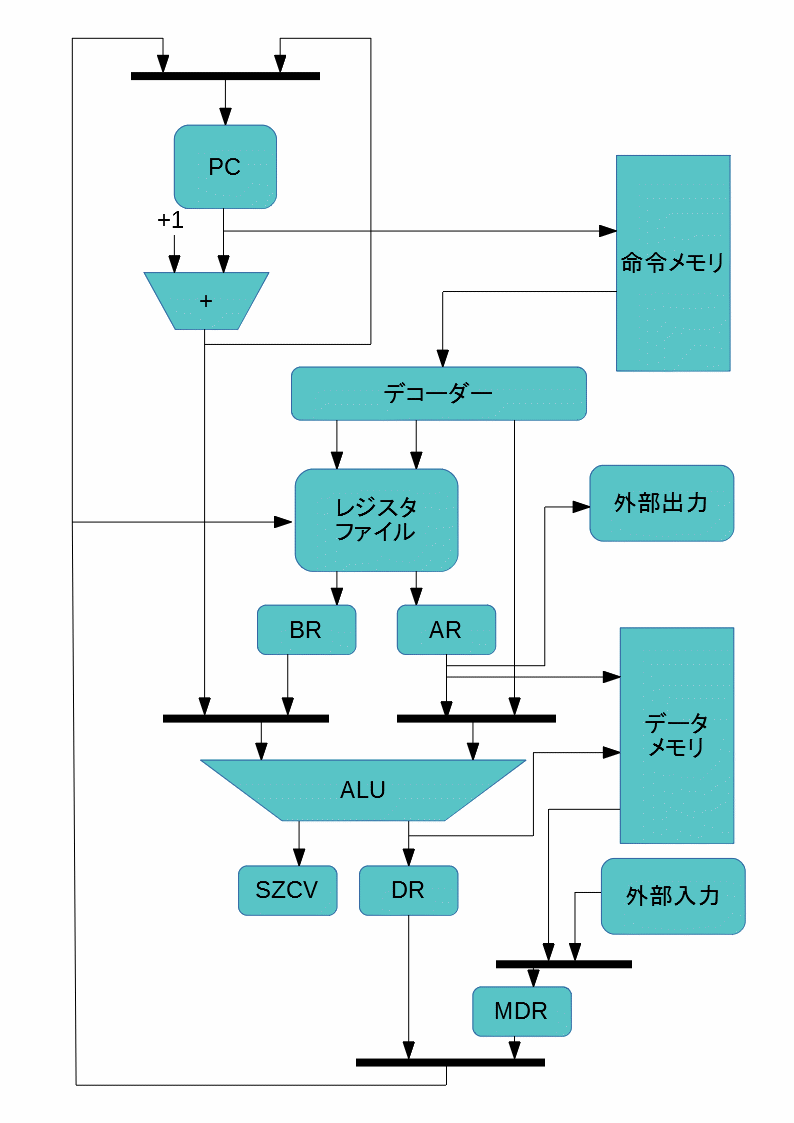
\includegraphics[width=120mm]{figures/data_flow.png}
\caption{ブロック図}
\label{fig:block}
\end{figure}

\subsubsection{各フェーズの動作}

\begin{description}
\item[p1] \mbox{} \\
PCの値の書き換えを行う。PCの保持するアドレスの命令を命令メモリからフェッチする(ただし、メモリから命令が実際に取り出されるのはp2)。
\item[p2] \mbox{} \\
メモリから取り出した命令をデコードする。レジスタファイルから読みだしたデータをAR、BRに格納する。
\item[p3] \mbox{} \\
ALUで演算を行い、結果をDRに格納する。外部出力命令なら、LEDに出力値が表示される。ロード・ストア命令では、ALUの演算結果をアドレスとしてデータメモリにアクセスする。ロード命令では、取り出したデータをMDRに格納し、ストア命令では、ARの値をメモリに書き込む(ただし、それらが実際に行われるのはp4)。
\item[p4] \mbox{} \\
SVCV、DRの値を更新する。
\item[p5] \mbox{} \\
MDRの値を更新する。分岐命令なら次のPCの値の書き換えはDRの値で行う。それ以外なら、PC+1で書き換える。必要なら、レジスタファイルへの書き込みを行う。
\end{description}

\subsection{性能}

回路サイズ・・・1374

最高動作周波数・・・61.76MHz

\section{分担状況}


\section{中間報告時点でのプロジェクトSIMPLEのタグ名}


\end{document}
